\documentclass[a4paper, 12pt]{article}
\usepackage{authblk}
\renewcommand{\Affilfont}{\footnotesize}
\title{Cabinet under Pressure: Survival Analysis of Peru’s Prime Ministers Since 1980}
\author[1,2]{ Jose Manuel Magallanes}
\affil{PULSO -Institute of Social Analytics and Strategic Intelligence\thanks{The author would like to thank the research assistants from PULSO-PUCP: Alexandra Porras, Alfredo Aro, Romina Loayza, Ivana Delgado, and Bruno Mago for their support  and dedication to this work.} and Department of Social Sciences, Pontificia Universidad Catolica del Peru, San Miguel 15088, Lima, Peru}
\affil[2]{University of Massachusetts-Amherst; University of Washington -Seattle; and Universidad Nacional Mayor de San Marcos-Lima}
\affil[*]{Corresponding author: jmagallanes@pucp.edu.pe}

\usepackage{tabularx,booktabs,threeparttablex,multirow,float}
\date{\today}  %% manually: \date{March 6, 2025} 
\usepackage[natbibapa]{apacite} %% for bibliography
\usepackage{rotating, graphicx} %% for rotating tables
\usepackage{adjustbox} % size of plots and tables
\usepackage{chngcntr}% section numbering
\usepackage{amssymb}
\usepackage{threeparttable}
\usepackage[table]{xcolor}
\usepackage{longtable}
\usepackage{array}        % For raggedright column specifier
\counterwithin{table}{section}\counterwithin{figure}{section}
\usepackage{Sweave}
\begin{document} % every "begin: needs and "end"
\Sconcordance{concordance:premieres.tex:premieres.Rnw:1 21 1 1 0 153 1 1 26 18 0 1 2 %
230 1 1 12 29 0 1 2 270 1}

\maketitle 
\begin{abstract}
This study examines the political durability of Peru’s Prime Ministers (PCM) since the country’s democratic return in 1980. While most studies treat ministers as a broad category, this analysis focuses on the PCM as a distinct figure within Peru’s hyper-presidential system—tasked with executive coordination and crisis absorption. Using survival analysis, we explore how political context, institutional conditions, and crisis dynamics shape the tenure of these key presidential appointees. Through a Cox proportional hazards model, we test the influence of presidential popularity, legislative fragmentation, cabinet reshuffles, and regime instability on the risk of early dismissal or resignation. The results illuminate how informal power-sharing and institutional fragility influence executive coordination in a hyper-presidential regime.
\end{abstract}




\section{Introduction} % * to unnumber

Although the 1979 Constitution of Peru defined the Prime Minister (PCM) merely as the president’s first minister—responsible for countersigning decrees and coordinating cabinet activity—subsequent legal and political developments have elevated the office to one that routinely performs head-of-government functions. These include drafting the policy agenda, negotiating confidence votes, and representing the executive in congressional interpellations. The PCM has thus come to serve as the president’s chief political shield. In periods of stable governance, the office facilitates legislative compromise and projects technocratic competence; in times of crisis, it functions as a “circuit-breaker”—a high-visibility scapegoat whose dismissal absorbs congressional discontent and helps preserve presidential tenure. Analyzing the determinants of PCM survival therefore sheds light on how Peru’s hyper-presidential system manages accountability, blame attribution, and policy coordination in the absence of strong political parties.
\begin{figure}[ht]
\centering
% \begin{adjustbox}%{width=0.9\textwidth,height=12cm,clip,trim=0cm 0cm 0cm 0cm} 
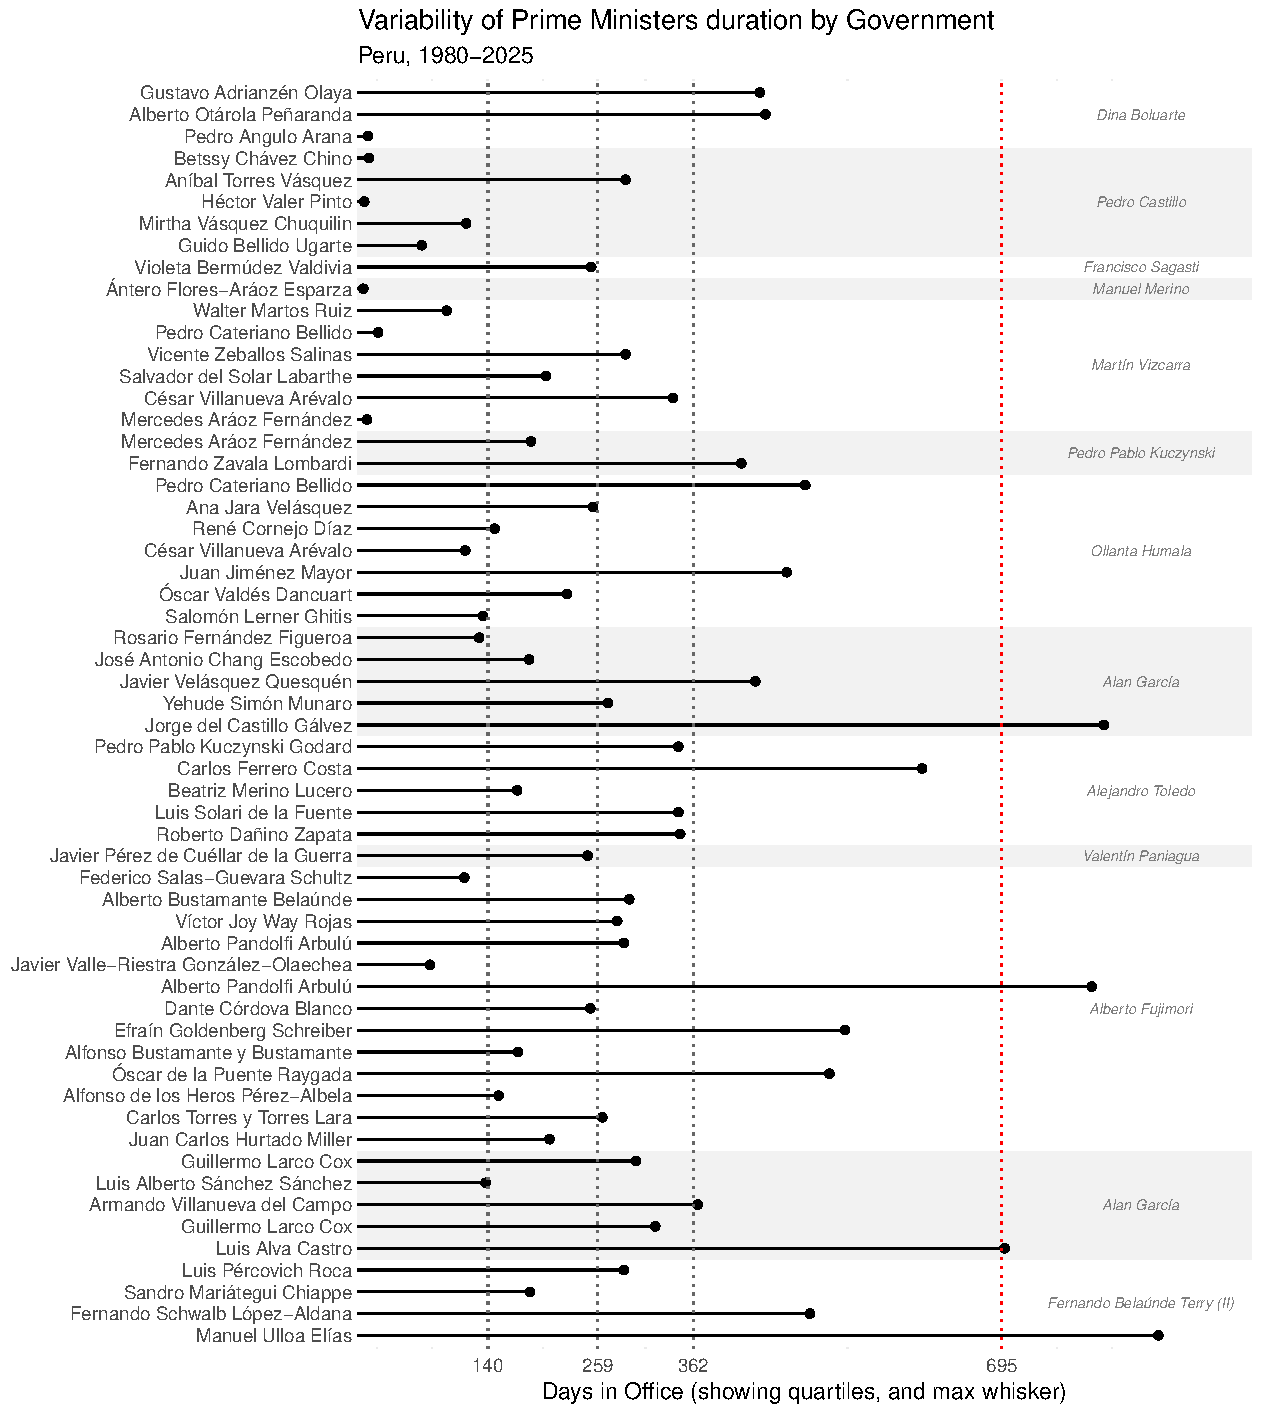
\includegraphics[width=0.85\textwidth]{durationLolli.pdf}
% \end{adjustbox}
\caption{Variability and Statistics Duration of PCMs in Perú from 1980 until 2025}  
\label{durationLolli} 
\end{figure}

The significance of this institutional role is underscored by the striking variation in PCM tenures. The median tenure since 1980 is just 254 days (approximately eight months), but durations vary widely (see Figure~\ref{durationLolli}). Ántero Flores-Aráoz lasted only six days in November 2020, whereas Manuel Ulloa served 864 days in the early 1980s, and Jorge del Castillo remained in office for 805 days during Alan García’s second term. This volatility persists even within single presidential administrations: three PCMs held the post during Pedro Castillo’s first five months, while Alberto Otárola remained in office for 440 days under Dina Boluarte. 

\begin{figure}[ht]
\centering
% \begin{adjustbox}%{width=0.9\textwidth,height=12cm,clip,trim=0cm 0cm 0cm 0cm} 
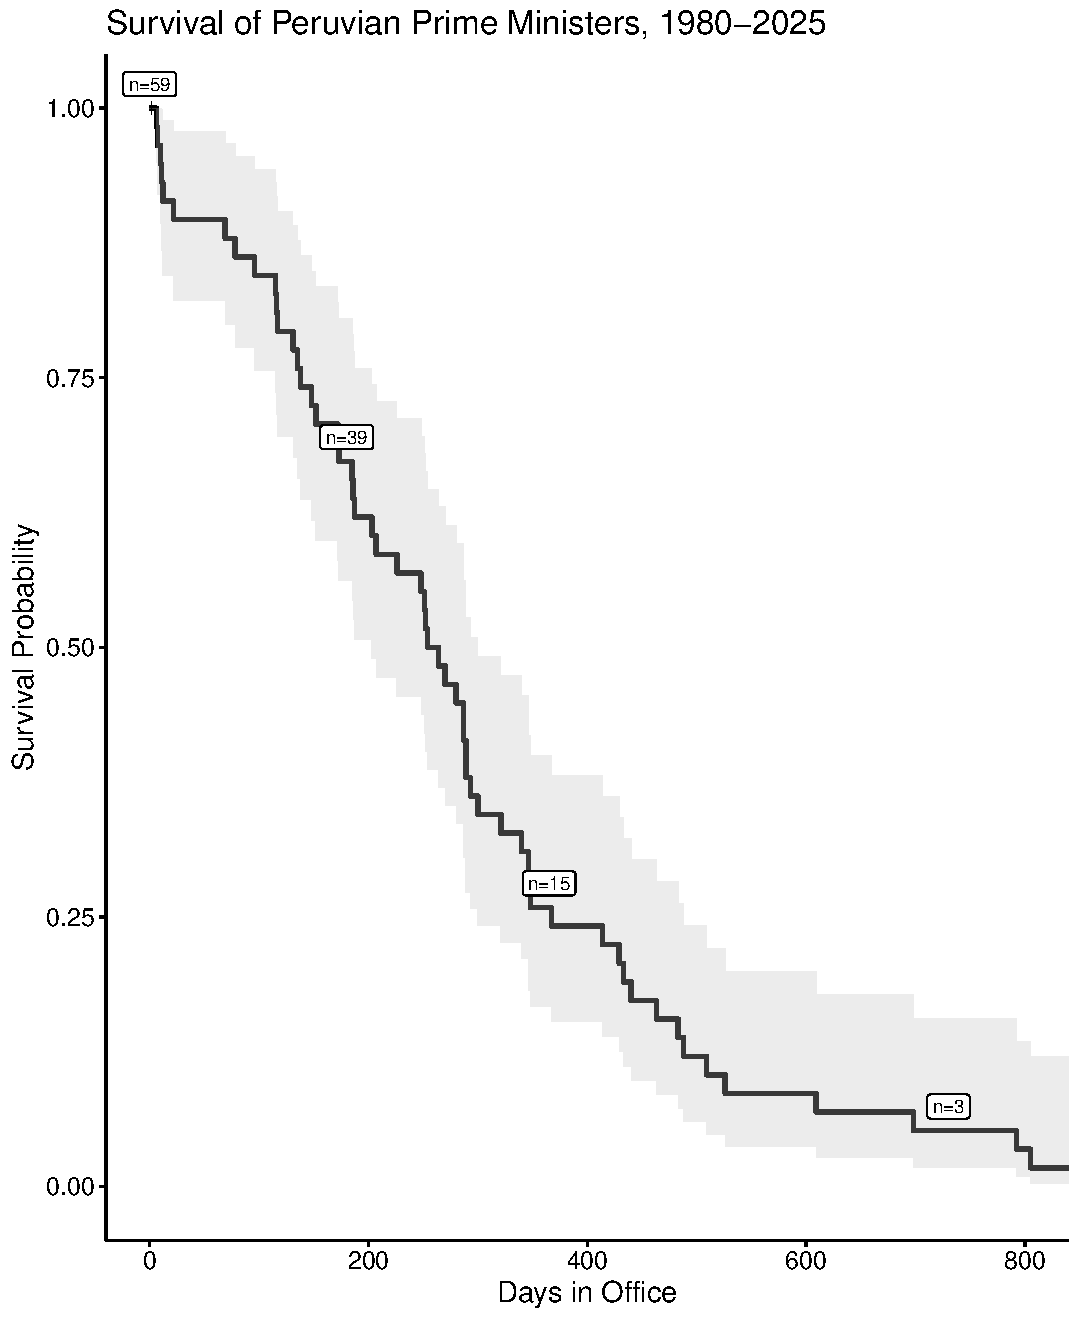
\includegraphics[width=0.85\textwidth]{kaplanDuration.pdf}
% \end{adjustbox}
\caption[Survival of Prime Ministers in Peru]{Kaplan-Meier survival estimate for Peruvian Prime Ministers, 1980--2025.}
\label{kaplanDuration} 
\end{figure}

The Kaplan-Meier survival estimate (Figure \ref{kaplanDuration}) illustrates this volatility. At the outset, all 58 PCMs are at risk. Within six months, only 40 remain; by one year, just 30 are still in office, and by the two-year mark, this number falls to 17. The survival probability drops below 50\% well before the one-year point and declines to around 20\% by year two. This pattern highlights how short-lived PCM tenures have become a structural feature of Peru’s political system rather than a sign of exceptional disruption. Understanding the forces behind such high turnover thus requires systematic analysis of the political, institutional, and situational factors that shape PCM survival—an inquiry taken up in the remainder of this study. Such inconsistency—despite ostensibly stable institutional rules—raises a central puzzle: which political, institutional, and situational factors shape the durability of Peru’s Prime Ministers?



\section{Background}\label{backg-tables} % label for crossref


\subsection{Understanding the PCM comparatively}

The role of the \textit{Presidente del Consejo de Ministros} (PCM) in Peru occupies a hybrid position: \textit{de jure} a minister within a presidential system, yet \textit{de facto} a coordinator of both cabinet and congressional relations—more akin to a prime minister in semi-parliamentary regimes. Article 124 of the Peruvian Constitution assigns the PCM formal responsibilities of coordinating the Council of Ministers and countersigning legislative acts \citep{republica_del_peru_constitucion_1993}. However, the role has informally expanded, particularly during crises, to absorb political blame and mediate executive-legislative conflict.

In the United Kingdom, the Prime Minister derives power from parliamentary majority and codified statutory provisions such as the \textit{Ministerial and Other Salaries Act 1975} \citep{united_kingdom_parliament_ministerial_1975} and the \textit{Standing Orders of the House of Commons} \citep{house_of_commons_standing_2024}. The Prime Minister leads both the executive and the parliamentary agenda.

Germany’s Federal Chancellor (\textit{Bundeskanzler}) is elected by the Bundestag under Article 63 of the Basic Law and exercises substantial agenda-setting power through the policy direction clause (\textit{Richtlinienkompetenz}, Article 65) \citep{federal_republic_of_germany_grundgesetz_1949}.

By contrast, the United States lacks a PCM-like figure. Executive power is concentrated in the President, as per Article II of the U.S. Constitution \citep{united_states_of_america_constitution_1787}. Legislative coordination is managed internally by congressional leaders, particularly the Majority and Minority Whips, whose authority stems from internal rules such as House Rule XXI and Senate Rule XXII \citep{us_house_of_representatives_rules_2023,us_senate_standing_2023}. These Whips are charged with vote counting, party discipline, and legislative scheduling—but act solely within the legislative branch.

Peru's PCM, uniquely, spans both domains. Though appointed and dismissed by the President, the PCM manages government program presentations and legislative negotiations, especially around confidence votes. This places the PCM between the partisan logic of legislative whips and the executive steering capacity of parliamentary heads of government.


\subsection{Evolution of the Prime Minister’s formal mandate} Peru’s Prime Minister (PCM) has migrated from a cabinet chair of convenience in the 1979 Constitution to a multisector policy coordinator and modernisation czar under the post‑2000 statutory framework.  Four legal milestones define that trajectory:


\begin{itemize}
\item 1979 Constitution (arts.215–218). The PCM presides over the Council of Ministers only when the President is absent; all appointments and dismissals rest with the President, who may chair the Council at will.  The PCM’s core duty is to secure majority support inside the cabinet for bills, decree‑laws, and matters of public interest. (Constitution 1979.)

\item 1993 Constitution (arts. 122–127). Retains presidential discretion over appointments but upgrades the PCM: he/she convenes the Council, signs legislative decrees, and must present the government programme and request a vote of confidence from Congress. (Democratic Constituent Congress 1993.)
\item Organic Law of the Executive Branch – LOPE 2007 (ch. II). Charges the PCM with proposing the government’s general objectives, coordinating multisectoral national policies—especially economic and social development—and supervising entities attached to the Presidency of the Council of Ministers. (Congress of the Republic 2007, LOPE.)
\item Law 29158 (2007) on Modernisation of the State (art.19). Designates the PCM the President’s highest‑trust agent, responsible for steering public‑sector modernisation and decentralisation across all tiers of government.  (Congress of the Republic 2007, Law 29158.)
\end{itemize}

Together these reforms turned the PCM from symbolic countersignatory into the President’s principal political shield and agenda gate‑keeper. See Table \ref{tab:pcm-mandate} for details on this evolution.

\begin{sidewaystable}[p]   % ‘p’ = put on its own float page
%\scriptsize
\centering
\caption{Evolution of the PCM’s formal mandate since 1979}
\label{tab:pcm-mandate}
\renewcommand{\arraystretch}{1.2}
\begin{tabularx}{\textheight}{@{}l X X X X l@{}}  % \textheight fits the rotated width
\toprule
\textbf{Legal framework} &
\textbf{Cabinet-chair role} &
\textbf{Policy-coordination powers} &
\textbf{Appointment \& dismissal} &
\textbf{Additional statutory duties} &
\textbf{Citation}\\
\midrule
1979 Constitution &
Chairs Council only when President absent; President may chair at will &
Secures majority consent for bills and decree-laws within the cabinet &
Exclusive presidential prerogative &
None specified beyond cabinet deliberations &
Const.\ 1979, arts.\ 215–218\\[4pt]

1993 Constitution &
Convenes Council; President may still chair &
Countersigns decrees; presents programme and confidence motion to Congress &
Exclusive presidential prerogative &
Must seek confidence votes &
Const.\ 1993, arts.\ 122–127\\[4pt]

LOPE 2007 &
PCM regularly chairs Council (President rarely attends) &
Proposes government objectives; coordinates multisector policies; supervises PCM-attached entities &
Unchanged &
Broad multisector supervision &
LOPE 2007, ch.\ II\\[4pt]

Law 29158 (2007) &
As per LOPE &
Leads State modernisation and decentralisation agenda &
Unchanged &
Strategic planning; inter-governmental coordination &
Law 29158, art.\ 19\\
\bottomrule
\end{tabularx}
\end{sidewaystable}

\subsection{Informal evolution: from symbolic coordinator to political operator}

The Prime Minister’s day‑to‑day leverage has always depended less on parchment rules than on shifting presidential strategies and congressional configurations.  Three sequential informal models can be distinguished:

\begin{itemize}

\item Symbolic coordinator (1980–1990).Under Belaunde and the first García administration the PCM remained a low‑profile chair; party‑fragmented congresses preferred dealing directly with sector ministers, and premiers changed whenever coalition arithmetic shifted.  Average tenure was 405 days, but the post was still viewed as an honorific stepping‑stone rather than a power centre.

\item Gate‑keeper in an autocratic presidency (1990 – 2000). Fujimori’s autogolpe (1992) sidelined Congress and broadened decree‑law rule.  The PCM became the sole bureaucratic filter for emergency economic decrees and IMF‑negotiated reforms; loyalty trumped expertise (e.g., Hurtado Miller, Pandolfi).  Although the decade’s mean tenure fell to $\approx 302$ days, variance shrank because Fujimori kept loyalists long until a policy pivot required a full cabinet refresh.

\item Floor‑manager and lightning rod (2001 – present). With the 1993 Constitution’s confidence‑vote mechanism now routinised, the PCM took on vote counting and crisis‑absorption roles.

\begin{itemize}

\item Coalition minority years (Toledo 2001‑06): premiers (e.g., Carlos Ferrero) traded ministerial posts for legislative backing.  

\item Party‑government years (García II 2006‑11): Jorge del Castillo doubled as APRA whip, illustrating the PCM’s partisan link function.  
\item Confrontational years (PPK, Vizcarra, Castillo): Congress weaponised interpellations; presidents sacrificed PCMs (Zavala 2017; Villanueva 2018; Bellido→Vásquez→Torres 2021‑22) to defuse censure threats or reset talks before the 28 July speech.  

\item Post‑2022 caretaker presidency: Dina Boluarte retained Alberto Otárola for 440 days to project continuity amid unrest, showing the PCM as stability signal.
\end{itemize}
\end{itemize}


Across these phases, two informal prerogatives emerged:

\begin{itemize}
\item Negotiator‑in‑chief. Modern PCMs draft the annual Mensaje a la Nación, map votes for confidence motions, and lobby party spokespeople—tasks never spelled out in LOPE.

\item High‑visibility “circuit‑breaker.” Presidents now time reshuffles to absorb blame for corruption scandals (e.g., Saavedra 2016 education dispute; Chávarry 2019 judicial scandal) or economic shocks, banking on a short‑term boost in approval.

\end{itemize}

These unwritten practices explain why Prime‑Ministerial exits cluster around scandals, protests, and the July speech window—patterns the survival analysis in Section 4 explicitly models.


\subsection{Prime‑Ministerial tenure across political periods}

Peru’s Prime‑Ministerial tenure remains volatile, but volatility itself is not uniform across eras.  Using the verified dataset of 57 spells (1980–2025), Table \ref{tab:durationPerEra} summarises the distribution by political period.  The Fujimori decade exhibits the shortest average tenure (302 days) yet also the narrowest spread, reflecting the concentration of presidential power; the immediate post‑transition years average roughly 405 days, while the post‑2000 era shows the shortest median (232 days) and the widest range as presidents cycle through PCMs to manage fragmented congresses and serial crises.



\begin{table}[!h]
\centering
\caption{Duration in Days by era\label{tab:durationPerEra}}
\centering
\begin{threeparttable}
\begin{tabular}[t]{lrrrrr}
\toprule
Era & count & mean & min & max & range\\
\midrule
A. Belaunde to Garcia & 9 & 405.44 & 138 & 864 & 726\\
B. Fujimori & 13 & 302.08 & 78 & 792 & 714\\
C. Paniagua to Boluarte & 37 & 240.89 & 2 & 805 & 803\\
\bottomrule
\end{tabular}
\begin{tablenotes}[para]
\item \textit{Source: } 
\item author calculations from official appointment resolutions and El Peruano archives.
\end{tablenotes}
\end{threeparttable}
\end{table}

\section{Conceptual Framework: Explaining PCM Survival}\label{concepframe}

This section synthesizes insights from the preceding background analysis to identify the main mechanisms likely to drive Prime Ministerial survival in Peru's political system. As shown in Sections 2.1 to 2.4, the PCM functions in a hybrid institutional role—legally subordinate to the President but often tasked with managing congressional coordination and absorbing political blame. Unlike portfolio ministers, the PCM plays a coordination and blame management role at the center of executive-legislative interaction. This structural ambiguity invites vulnerability to shifts in both formal and informal dynamics.

First, the historical \textbf{informal evolution} of the PCM role (Section 2.3) reveals a pattern where the office becomes a focal point for defusing crises. From this, we derive the importance of \textbf{Political Shocks} as a key covariate: resignations or reshuffles often follow scandals or protests.

Second, the PCM’s effectiveness often depends on the \textbf{President's popularity} and authority (Section 2.3 and 2.4). When approval falls, presidents are more likely to replace PCMs to reassert control or appease public dissatisfaction---justifying the inclusion of \textbf{Presidential Approval} as a time-varying covariate.

Third, as Section 2.1 and 2.4 emphasize, Peru’s fragmented legislature frequently weakens coalition durability, forcing PCMs to engage in high-stakes legislative negotiation. This supports the inclusion of \textbf{Legislative Fragmentation} as a predictor of PCM risk.

Fourth, the background section highlights how confidence votes and reshuffles cluster around symbolic moments, such as the July 28 address. This justifies including a \textbf{Critical Periods} variable tied to the calendar.

Fifth, the informal role of PCMs as ``technocratic shields'' or outsiders suggests that the \textbf{Technocratic Profile} of the individual minister could affect their disposability, especially under outsider presidencies.

Finally, Section 2.3 distinguishes the authoritarian dynamics of the Fujimori regime from other eras. Under this logic, \textbf{Regime Type} (democratic vs. autocratic) functions as a contextual variable shaping the overall hazard baseline.

These six factors emerge inductively from the Peruvian institutional context and form the backbone of the survival analysis presented in later sections.

% \begin{figure}[h!]
%   \centering
%   \includegraphics[width=0.8\textwidth]{dag_pcm_survival.png}
%   \caption{Directed Acyclic Graph (DAG): Hypothesized Drivers of PCM Survival}
%   \label{fig:dag_pcm_survival}
% \end{figure}


\section{Literature Review}\label{sec:letrev}


This literature review contextualizes the six drivers of PCM survival identified in the conceptual framework (Section \ref{concepframe}), situating them within broader comparative and regional findings. Comparative studies have consistently identified Peru as an outlier in cabinet turnover, with unusually short ministerial tenures even by regional standards \citep{martinez-gallardo_out_2012, gozzer_duracion_2021}. For instance, \citet{martinez-gallardo_out_2012} shows that Peru's cabinets exhibit among the highest turnover rates in Latin America, with \citet{gozzer_duracion_2021} confirming similar volatility at the sectoral level in health ministries. Before examining each factor, it is important to recognize that Peru's cabinet instability is not a recent development, but a structural feature of its political system. This volatility motivates the search for proximate, theoretically grounded covariates to explain PCM survival in a highly unstable institutional context.


\subsection{Political Shocks and Crisis Events}

Peru’s modern history is marked by repeated, acute political shocks that have profoundly shaped the stability of cabinets and the role of PCMs:

\begin{itemize}
  \item \textbf{The Extreme Political Violence (1980s–1990s):} Armed violence by Sendero Luminoso and the MRTA placed sustained pressure on Peru’s executive capacity. The Peruvian state oscillated between heavy-handed repression and strategic inaction, often failing to formulate a coherent institutional response. Cabinet instability during this period reflected not only security challenges but also political fragmentation, as successive administrations struggled to maintain authority amid systemic violence.
  \item \textbf{Hyperinflation and Economic Collapse (late 1980s):} Under García’s first term, inflation soared and protests escalated, fueling cabinet turnover amid a broader legitimacy crisis.
  \item \textbf{Neoliberal Adjustment (1990s):} The ``Fujishock'' program implemented under Fujimori provoked social resistance and political fragmentation, prompting frequent ministerial replacements.
  \item \textbf{Congress Dissolution (1992, 2019):} Fujimori's autogolpe and Vizcarra’s congressional shutdowns restructured political bargaining and undermined cabinet continuity.
  \item \textbf{Presidential Impeachments and Removals (2000, 2018–2022):} Fujimori’s fall, Vizcarra’s forced exit, and Castillo’s abrupt ouster were all accompanied by PCM reshuffles and resignations.
\end{itemize}

These cases illustrate that in Peru, political shocks are not exceptional disturbances but recurrent inflection points in executive–legislative dynamics. They often expose the limited institutional capacity of governments to manage sudden disruptions without resorting to cabinet change. Comparative research reinforces this pattern. As \citet[609]{camerlo_minister_2015-1} observe, ``cabinet turnover is a flexible mechanism presidents use to defuse crises, absorb blame, and adjust to political turbulence.'' Scandals and protests also differ in their temporal logic. As \citet[611]{camerlo_minister_2015-1} show, ``presidents are more likely to dismiss ministers in response to scandals early in the term, and in response to protests closer to the next election.'' In Peru’s hyper-presidential context, such shocks are absorbed through cabinet reshuffles, where Prime Ministers serve as expendable buffers. As \citet[7-9]{dargent_technocracy_2014} notes, technocrats in Latin America are often appointed for their market legitimacy, but their lack of political embeddedness makes them ideal targets in moments of institutional stress.




\subsection{Institutional Determinants: Approval, Fragmentation, Regime Type}

PCM risk is shaped by institutional context. Presidential approval levels matter in both parliamentary and presidential regimes \citep{fischer_duration_2012}. However, low approval is not always driven by objective crises. In Peru, presidents have often seen their approval erode over time due to political style, poor media management, or antagonistic relations with Congress—even in the absence of acute shocks.

This trend has been noted across multiple administrations. As \citet{tanaka_democracia_2005} argues, declining presidential approval in Peru often stems from a broader crisis of representation and weak party linkages, rather than specific policy failures or scandals. For example, García's second term saw approval decline even without economic crisis, while Alejandro Toledo’s consistently low ratings were attributed more to communication failures than specific scandals \citep{tanaka_democracia_2005, levitsky_latin_1999}.

Legislative fragmentation reduces durability by raising coordination costs \citep{huber_replacing_2008}. In fragmented legislatures, prime ministers must navigate more complex negotiations to secure majority backing, which increases the probability of legislative deadlock or failed votes of confidence. This dynamic weakens the executive’s policy coherence and forces presidents to reshuffle PCMs as a political concession or to reset stalled agendas. In Peru, this fragmentation is rooted in the collapse of the party system during and after the Fujimori era. The weakening of traditional parties and the rise of personalist movements undermined partisan discipline in Congress, making legislative coordination more unstable \citep{levitsky_latin_1999, tanaka_democracia_2005, garcia_marin_fragmentacion_2024}. As \citet{garcia_marin_fragmentacion_2024} argues, this fragmentation is compounded by the proliferation of weak or regional parties and low levels of institutionalization, which encourage legislators to abandon their electoral banners and form ad hoc caucuses. These dynamics erode party cohesion and complicate executive negotiation. As a result, high legislative atomization has often coincided with short PCM spells and volatile cabinet turnover, reflecting the difficulty of sustaining governing coalitions in multiparty settings without stable partisan anchors.

Regime variation also matters: cabinets survive longer in parliamentary systems and less under autocratic concentration, as in the Fujimori period \citep{perez-linan_presidential_2007, garcia_marin_fragmentacion_2024}. Fujimori marks a critical point of institutional transformation. His 1992 autogolpe suspended Congress and the Constitution, replacing party-based coordination with technocratic governance and decree-based policymaking. This shift enabled greater executive autonomy but dismantled mechanisms of horizontal accountability. The PCM became increasingly subordinated to presidential discretion, reshaping the logic of cabinet stability away from coalition management and toward intra-executive loyalty. In the context of survival analysis, this regime shift alters the baseline hazard: under democratic periods, PCM tenure risk is more responsive to approval and fragmentation, while under Fujimori's autocratic model, survival reflects internal alignment with the executive rather than legislative negotiation or public legitimacy.


\subsection{Ministerial Profiles and Technocratic Survival}

Individual attributes of ministers—especially their technocratic background or outsider status—can shape their survival in office. \citet{escobar-lemmon_coming_2010} argue that technocrats may lack the partisan protection that buffers career politicians from dismissal, making them more vulnerable to turnover in polarized or unstable environments. \citet{alexiadou_commitment_2019} further demonstrate that technocratic appointments are more likely during periods of economic crisis, when credibility is paramount, but such ministers often lack embedded networks within governing coalitions.

In Peru, the recurrent use of technocrats reflects both institutional weakness and political opportunism. As \citet{carreras_presidentes_2013} notes, outsider presidents like Fujimori and Kuczynski frequently turned to technocratic PCMs to signal competence and distance from discredited party elites. However, these figures—often drawn from academia, international institutions, or business—are expendable once the political calculus shifts. Many of them bring traits associated with successful private careers, such as managerial credentials, international networks, and policy expertise, which boost their short-term credibility but do not necessarily offer them political protection. \citet[pp.~45--48]{dargent_technocracy_2014} emphasizes that technocrats derive legitimacy from their reputational capital and market credibility rather than from partisan loyalty, making them simultaneously valuable in crisis and disposable in negotiation. As he notes, ``technocrats are not protected by party loyalties or legislative networks; their authority is grounded in expertise, which makes them vulnerable when politics reasserts itself.''

The survival of technocratic PCMs in Peru thus hinges not only on individual expertise but on institutional context. In fragmented or highly politicized environments, lack of embeddedness may increase their hazard rate. The latent technocrat index included in this study captures this profile and tests whether outsider expertise—absent partisan insulation—correlates with shorter tenure.


\subsection{Critical Periods and Strategic Timing}

Ministers are not dismissed uniformly across time. Political science recognizes the role of electoral and institutional calendars in shaping reshuffle windows (e.g., annual messages, budget votes). In Peru, the July 28 address often anchors symbolic resets, justifying the inclusion of a speech-window dummy.

Beyond institutional rituals, \citet[611]{camerlo_minister_2015-1} demonstrate that the timing of shocks interacts with the president’s electoral horizon. ``Presidents are more likely to dismiss ministers in response to scandals early in the term, and in response to protests closer to the next election.'' For non-reelectable presidents, this pattern reverses. These dynamics also apply to ministerial agency: ``ministers are more likely to resign in response to protests when they are eligible for reelection and to leave in response to scandals when reelection is not possible'' \citep[611]{camerlo_minister_2015-1}.

This interaction between shock type, calendar, and political incentives supports the inclusion of time-varying covariates in the survival model. These account for both scheduled reshuffle windows and critical events that can accelerate PCM exits.


\subsection{Synthesis and Gaps}

While existing literature provides robust evidence on the impact of political shocks, institutional fragmentation, and technocratic appointments, these factors are typically analyzed in isolation or within cross-national comparisons. Few studies integrate all six drivers of ministerial stability—political, institutional, and individual-level—into a single country-specific model. Moreover, most contributions examine ``ministers'' as a broad category—often focusing on sectoral portfolios or aggregated cabinet trends—without distinguishing the PCM's unique institutional role. Unlike other ministers, the PCM in Peru serves as a central political operator who coordinates executive-legislative relations and often absorbs political blame during periods of instability. This strategic placement within the presidential team makes the PCM especially sensitive to crisis dynamics and power shifts in ways that traditional ministerial models may overlook.

This study contributes by developing a unified survival framework tailored to Peru’s distinctive institutional configuration, with a specific focus on the presidency's key operator: the PCM. It incorporates not only regime type and presidential approval but also calendar timing, fragmentation, and technocratic profile—capturing how formal and informal rules interact in a hyper-presidential, weakly institutionalized setting. By embedding these dynamics in a Cox proportional hazards model, the study extends prior findings on Latin America’s executive volatility and offers a disaggregated, temporally sensitive account of cabinet duration in Peru.





\section{Data and Methods}

\subsection{Dataset construction}


This study draws on an event-history dataset covering all 57 Prime-Ministerial spells between 28 July 1980 and 8 May 2025. Each spell corresponds to a continuous period during which a single individual served as Prime Minister (PCM), from their swearing-in to dismissal or resignation. Gustavo Adrianzén’s ongoing tenure is treated as right-censored as of 8 May 2025.

The explanatory variables are grouped into two categories:

\textbf{(a) Non–time-varying variables}, which remain constant throughout a PCM’s spell. These include:

\begin{itemize}
    \item \textit{Technocratic profile}: A latent trait index derived from five binary indicators: (i) absence of previous electoral participation, (ii) graduate degree obtained abroad, (iii) relevant private sector experience, (iv) academic background, and (v) having a degree other than law. These variables reflect the literature on technocratic appointments (Carreras, 2013; Alexiadou, 2016; Escobar-Lemmon \& Taylor-Robinson, 2010). We estimate a continuous score using Latent Trait Modeling (LTM), validated through PCA and EFA. The continuous index is used in all Cox regressions; a binary split at the median is used for descriptive survival plots.
    
    \item \textit{Fujimori regime dummy}: A fixed indicator for spells that occurred during the presidency of Alberto Fujimori (April 1990 to July 2000), capturing the autocratic institutional context of that period.
\end{itemize}

\textbf{(b) Time–varying variables}, which may change within a PCM’s tenure and thus require finer temporal resolution. These include:

\begin{itemize}
    \item \textit{Presidential approval}: Quarterly approval ratings from Ipsos Perú;
    \item \textit{Legislative fragmentation}: Measured via the effective number of parties (ENP), calculated from congressional seat shares;
    \item \textit{Censure motions}: A binary indicator coded 1 if a motion for interpellation or censure was active during the interval;
    \item \textit{Economic shock}: Equals 1 if quarterly GDP growth is negative;
    \item \textit{Speech window}: Equals 1 if the interval includes ±45 days around the annual \textit{Mensaje a la Nación} on 28 July.
\end{itemize}

To correctly update these time-varying covariates mid-tenure, we adopt the Andersen–Gill (AG) counting-process framework, splitting each PCM spell into annual intervals anchored on 28 July. This allows each time-varying covariate to update in a temporally valid way while preserving the structure of the Cox partial likelihood. Robust standard errors are clustered by PCM to account for repeated observations.

\begin{sidewaystable}[p]
%\scriptsize
\centering
\caption{Variables, Operationalization, Sources, and Literature}
\label{tab:variables}
\begin{tabular}{
  >{\raggedright\arraybackslash}p{3cm} 
  >{\raggedright\arraybackslash}p{3.5cm} 
  >{\raggedright\arraybackslash}p{6cm} 
  >{\raggedright\arraybackslash}p{2.5cm} 
  >{\raggedright\arraybackslash}p{4cm}
}
\toprule
\textbf{Category} & \textbf{Variable} & \textbf{Operationalization} & \textbf{Source} & \textbf{Literature} \\
\midrule

\multicolumn{5}{l}{\textit{Non–Time-Varying Covariates}} \\
\midrule

Profile & Technocrat Index & Latent trait score from five binary indicators: no electoral experience, foreign graduate education, private sector or academic background, and non-law degree. Estimated via LTM and validated via PCA and EFA. & CVs and secondary sources & Carreras (2013); Alexiadou (2016); Escobar-Lemmon \& Taylor-Robinson (2010); Bersch et al. (2017) \\

Regime & Fujimori & 1 if PCM served between 5 April 1990 and 28 July 2000 & Author coding & Pérez-Liñán (2007); Fischer et al. (2012) \\

\midrule
\multicolumn{5}{l}{\textit{Time–Varying Covariates}} \\
\midrule

Congress & ENP & Quarterly effective number of parties (seat share) & JNE seat records & Huber \& Martínez-Gallardo (2008); Martínez-Gallardo (2012) \\

Congress & Censure motion & 1 if interpellation or censure motion was tabled during interval & Congressional Journal & Camerlo \& Pérez-Liñán (2015); Dewan \& Dowding (2005) \\

Presidency & Approval & Quarterly presidential approval (\%) & Ipsos Perú & Samuels \& Shugart (2003); Fischer et al. (2012) \\

Calendar & Speech window & 1 if within ±45 days of 28 July & Author calculation & This study (informal calendar logic) \\

Economy & GDP shock & 1 if quarterly GDP growth is negative & BCRP & González-Bustamante \& Olivares (2016) \\

\bottomrule
\end{tabular}
\end{sidewaystable}



%%%

\subsection{Computing Time Invariant Covariates}

\subsubsection{The regime epoch}

\subsubsection{Latent Trait Modeling of Technocratic Profile}

To operationalize the technocratic orientation of Prime Ministers (PCMs), we estimate a latent trait model using three binary indicators grounded in the literature on technocratic appointments in Latin America and beyond: (i) absence of prior electoral participation, (ii) possession of a graduate degree from a foreign university, and (iii) relevant private sector experience. Each trait captures a distinct aspect of the technocratic profile.

The absence of electoral participation reflects political independence, a hallmark of technocratic appointments, particularly under outsider presidencies and in contexts of weak party institutionalization \citep{escobar-lemmon_coming_2010, carreras_presidentes_2013}. A foreign graduate degree signals technical training and elite socialization, often aligned with global policy norms \citep{alexiadou_ideologues_2016, camp_mexicos_2002}. Private sector experience, particularly in consulting, banking, or corporate management, signals not only managerial competence but also autonomy from state careers. Technocrats often derive their legitimacy from reputational capital earned outside the public sector. As Alexiadou and Günaydin \citep{alexiadou_commitment_2019} argue, technocrats are professionals motivated by expertise and external reputation, who “typically aim at better employment prospects by building a positive reputation in their professional field.” This complements Dargent’s \citep{dargent_technocracy_2014} observation that many Latin American technocrats enter the state from positions of market-based credibility rather than political dependence. Similar arguments are found in earlier studies linking private sector expertise to technocratic authority in reform-oriented administrations \citep{centeno_democracy_1997, weyland_politics_2021}.

We model these three traits as manifestations of a continuous latent technocratic dimension using a two-parameter logistic latent trait model (2PL), estimated with the \texttt{ltm} package in R. The model allows for item-specific variation in difficulty and discrimination, and assumes that the probability of endorsing each trait increases with the unobserved technocratic score.

As you can see in Table \ref{tab:ltm_parameters}, estimation results show that “no prior electoral experience” and “foreign graduate degree” are strong discriminators (discrimination parameters > 2.1), while “private sector experience” has lower discrimination (1.17) but higher difficulty (0.91), suggesting it marks the upper end of the technocratic scale. Figure \ref{fig:iccplot} presents item characteristic curves (ICCs) for the three indicators.

Individual-level scores are computed using expected a posteriori (EAP) estimation and assigned to PCMs by matching response patterns to model-derived scores. The resulting technocratic index ranges from approximately --1.5 to +2.6, with higher scores reflecting stronger technocratic profiles. The index is strongly correlated with PCA- and EFA-based indices ($r > 0.95$), and tracks well with clusters identified via unsupervised classification.

The continuous LTM-based index is used in Cox proportional hazards models to assess its effect on PCM survival. For descriptive Kaplan–Meier analysis, we also construct a binary version based on the median split.

% latex table generated in R 4.4.0 by xtable 1.8-4 package
% Thu May 15 19:42:25 2025
\begin{table}[ht]
\centering
\caption{Latent Trait Model: Discrimination and Difficulty Parameters} 
\label{tab:ltm_parameters}
\begin{tabular}{lrrrc}
  \hline
Parameter & Estimate & Std. Error & z-value &  \\ 
  \hline
\addlinespace
\multicolumn{4}{l}{\textit{Discrimination Parameters}} \\[-15pt] &  &  &  &  \\ 
  No electoral participation & 2.18 & 1.62 & 1.35 &  \\ 
  Foreign degree & 2.16 & 1.57 & 1.37 &  \\ 
  Private sector experience & 1.20 & 0.64 & 1.87 & . \\ 
  \addlinespace
\multicolumn{4}{l}{\textit{Difficulty Parameters}} \\[-15pt] &  &  &  &  \\ 
  No electoral participation & 0.30 & 0.23 & 1.27 &  \\ 
  Foreign degree & 0.49 & 0.26 & 1.87 & . \\ 
  Private sector experience & 0.92 & 0.44 & 2.07 & * \\ 
   \addlinespace
\addlinespace
\multicolumn{5}{l}{\footnotesize\textit{Model fit: log-likelihood = -97; AIC = 205.02; BIC = 216.95.}} \\\multicolumn{5}{l}{\footnotesize\textit{Estimated via BFGS optimization.}} \\\multicolumn{5}{l}{\footnotesize\textit{Convergence: Yes (grad = 0.00055906).}} \\\multicolumn{5}{l}{\footnotesize\textit{Integration: Gauss-Hermite with 21 points.}} \\\hline 
 \multicolumn{5}{l}{\textit{Note}: $^{*} p<0.05$, $^{.} p<0.10$} \\ 
 \hline
\end{tabular}
\end{table}


\begin{figure}[ht]
\centering
% \begin{adjustbox}%{width=0.9\textwidth,height=12cm,clip,trim=0cm 0cm 0cm 0cm} 
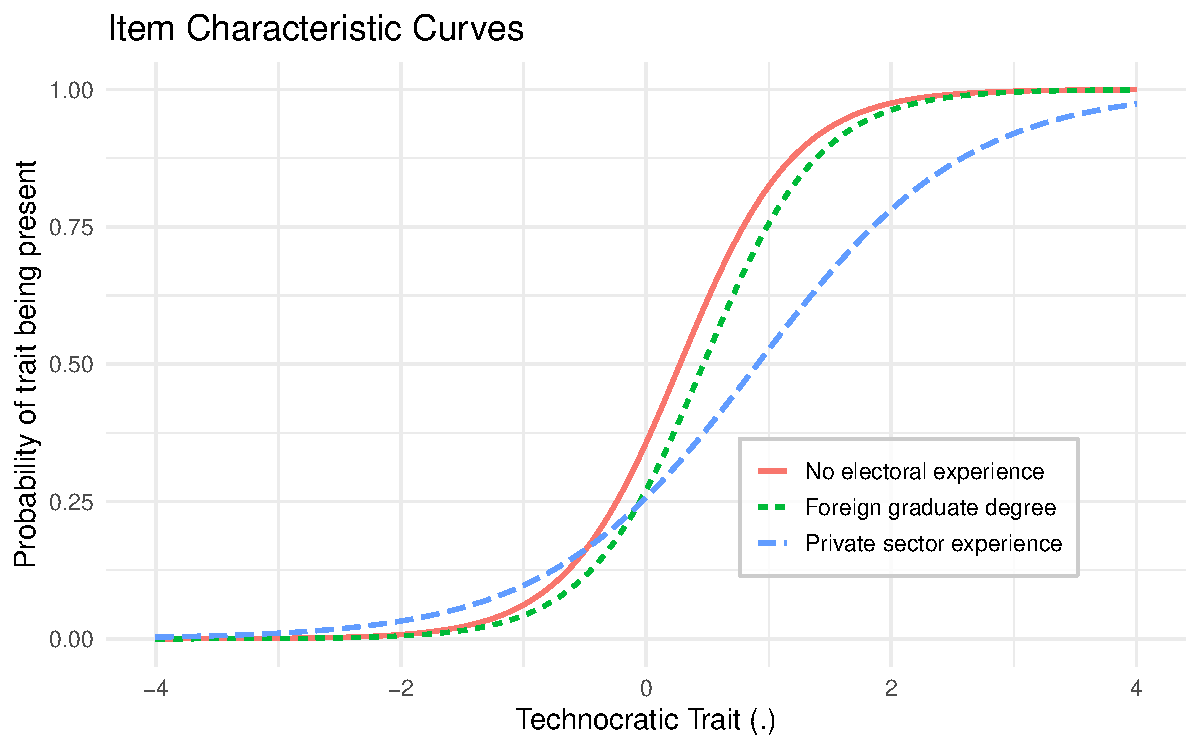
\includegraphics[width=\textwidth]{iccplot.pdf}
% \end{adjustbox}
\caption{Variability and Statistics Duration of PCMs in Perú from 1980 until 2025}  
\label{fig:iccplot} 
\end{figure}



\subsection{Model specification}

The baseline estimation is a Cox proportional‑hazards model with shared frailty by presidential administration. Ties are handled with the Efron method, and robust standard errors are clustered on presidencies to absorb unobserved style differences.

We express the hazard for PCM spell \(i\) under president \(j\) at time \(t\) as:

\[
  h_{ij}(t \mid X_i(t), u_j)
    = h_0(t) \exp\bigl(\beta^{\mathsf{T}}X_i(t) + u_j\bigr),
  \quad u_j \sim \mathcal{N}(0,\sigma^2),
\]


\paragraph{Explanation of terms}
\begin{itemize}
  \item $h_{ij}(t \mid X_i(t), u_j)$: the hazard rate for spell $i$ under president $j$ at time $t$, i.e., the instantaneous risk of exit.
  \item $h_0(t)$: the baseline hazard function, representing the underlying risk when all covariates are zero.
  \item $X_i(t)$: the vector of (possibly time-varying) covariates for spell $i$, including ENP, approval, GDP shocks, and the speech-window dummy.
  \item $\beta$: the vector of regression coefficients quantifying each covariate’s effect on the log-hazard.
  \item $\beta^\top X_i(t)$: the linear predictor (log-relative hazard) combining covariates and coefficients.
  \item $u_j$: the shared-frailty term (a random effect) for administration $j$, capturing unobserved presidency-level heterogeneity.
  \item $u_j \sim \mathcal{N}(0,\sigma^2)$: indicates $u_j$ follows a normal distribution with mean 0 and variance $\sigma^2$, where $\sigma^2$ measures unexplained variance across presidencies.
\end{itemize}


% The baseline estimation is a **Cox proportional‑hazards model with shared frailty by presidential administration**, implemented in R with the `coxme` package. Note that while `survival::coxph` supports simple frailty terms, the `coxme` package is required for estimating mixed‑effects Cox models with normally distributed random effects (shared frailty) across presidencies.








\section{Results}

% Table created by stargazer v.5.2.3 by Marek Hlavac, Social Policy Institute. E-mail: marek.hlavac at gmail.com
% Date and time: Fri, May 16, 2025 - 23:53:43
\begin{table}[!htbp] \centering 
  \caption{} 
  \label{coxInvar} 
\begin{tabular}{@{\extracolsep{5pt}}lc} 
\\[-1.8ex]\hline 
\hline \\[-1.8ex] 
 & \multicolumn{1}{c}{\textit{Dependent variable:}} \\ 
\cline{2-2} 
\\[-1.8ex] & Survival in Office \\ 
\hline \\[-1.8ex] 
 regimeFujimori & $-$0.047 \\ 
  & (0.367) \\ 
  & \\ 
 technocrat\_trait\_ltm & 0.020 \\ 
  & (0.195) \\ 
  & \\ 
\hline \\[-1.8ex] 
Observations & 59 \\ 
R$^{2}$ & 0.0003 \\ 
Max. Possible R$^{2}$ & 0.998 \\ 
Log Likelihood & $-$180.447 \\ 
Wald Test & 0.020 (df = 2) \\ 
LR Test & 0.019 (df = 2) \\ 
Score (Logrank) Test & 0.019 (df = 2) \\ 
\hline 
\hline \\[-1.8ex] 
\textit{Note:}  & \multicolumn{1}{r}{$^{*}$p$<$0.1; $^{**}$p$<$0.05; $^{***}$p$<$0.01} \\ 
\end{tabular} 
\end{table} 


% 
% \subsection{Initial model}
% 
% <<echo=FALSE,results=tex>>=
% 
% library(survival)
% library(coxme)
% library(stargazer)
% # library(arrow)
% 
% 
% # 1. Load the AG intervals
% intervals_AG=arrow::read_parquet(file = "AG_intervals.parquet")
% 
% # 2. Fit the minimal “base” model: regime + speech, frailty by president
% fit_base_AG <- coxme(
%   Surv(interval_duration, event) ~ regime_fujimori + speech_window + (1 | presidentofExecutive),
%   data = intervals_AG,
%   ties = "efron"
% )
% fit=fit_base_AG
% s=summary(fit_base_AG)
% 
% 
% # --- Random effect ---
% # --- Random Effects ---
% re_sd <- round(s$random[["sd"]][1], 5)
% re_var <- round(re_sd^2, 8)
% 
% # --- Random Effects Model Fit (from s$chi) ---
% chi_df <- round(as.data.frame(s$chi), 4)
% 
% # chi_df rows: "Integrated", "Penalized"; columns: Chisq, df, p, AIC
% 
% # --- Full Model Fit ---
% loglik_val <- round(logLik(fit)[1], 2)
% df_val     <- attr(logLik(fit), "df")
% aic_val    <- round(AIC(fit), 2)
% 
% # --- Fixed Effects ---
% fe <- s$coefficients
% fe_out <- apply(fe, 1, function(row) {
%   coef <- round(row["coef"], 4)
%   hr   <- round(exp(row["coef"]), 4)
%   se   <- round(row["se(coef)"], 4)
%   z    <- round(row["z"], 2)
%   pval <- round(2 * (1 - pnorm(abs(z))), 3)
%   sprintf("%s & %.4f & %.4f & %.4f & %.2f \\quad %.3f \\\\", 
%           rownames(fe)[which(fe[, "coef"] == row["coef"])],
%           coef, hr, se, z, pval)
% })
% 
% # --- Output LaTeX file ---
% out_file <- "coxme_summary.tex"
% 
% cat(
% "\\begin{table}[ht]
% \\centering
% \\begin{threeparttable}
% \\caption{Cox Mixed-Effects Model Summary}
% \\label{tab:coxme_auto}
% \\begin{tabular}{lllll}
% \\toprule
% \\multicolumn{5}{l}{\\textbf{Random Effects}} \\\\
% \\midrule
% Group & Variable & SD & Variance & \\\\
% presidentofExecutive & Intercept & ", re_sd, " & ", re_var, " & \\\\
% \\\\
% \\multicolumn{5}{l}{\\textbf{Random Effects Model Fit (LRT)}} \\\\
% \\midrule
% Method & Chisq & df & p & AIC \\\\
% Integrated loglik & ", chi_df[1, "Chisq"], " & ", chi_df[1, "df"], " & ", chi_df[1, "p"], " & ", chi_df[1, "AIC"], " \\\\
% Penalized loglik & ", chi_df[2, "Chisq"], " & ", chi_df[2, "df"], " & ", chi_df[2, "p"], " & ", chi_df[2, "AIC"], " \\\\
% \\\\
% \\multicolumn{5}{l}{\\textbf{Full Model Fit}} \\\\
% \\midrule
% Statistic & & & & \\\\
% Penalized log-likelihood & & & & ", loglik_val, " \\\\
% Degrees of freedom & & & & ", df_val, " \\\\
% AIC & & & & ", aic_val, " \\\\
% \\\\
% \\multicolumn{5}{l}{\\textbf{Fixed Effects}} \\\\
% \\midrule
% Variable & Coef & exp(Coef) & SE(Coef) & z \\quad p \\\\
% ", paste(fe_out, collapse = "\n"), "
% \\bottomrule
% \\end{tabular}
% \\begin{tablenotes}
% \\footnotesize
% \\item \\textit{Note}: Coefficients are from a Cox proportional hazards mixed-effects model with a random intercept. SD = standard deviation of random effect. Variance = SD\\textsuperscript{2}.
% \\item \\textit{exp(Coef)} is the hazard ratio. p-values are based on z-tests.
% \\item Significance: * p<0.1; ** p<0.05; *** p<0.01
% \\end{tablenotes}
% \\end{threeparttable}
% \\end{table}
% ", file = out_file)
% 
% @
% 
% \begin{table}[ht]
\centering
\begin{threeparttable}
\caption{Cox Mixed-Effects Model Summary}
\label{tab:coxme_auto}
\begin{tabular}{lllll}
\toprule
\multicolumn{5}{l}{\textbf{Random Effects}} \\
\midrule
Group & Variable & SD & Variance & \\
presidentofExecutive & Intercept &  0.01999  &  0.0003996  & \\
\\
\multicolumn{5}{l}{\textbf{Random Effects Model Fit (LRT)}} \\
\midrule
Method & Chisq & df & p & AIC \\
Integrated loglik &  1.4  &  3  &  0.7061  &  -4.6  \\
Penalized loglik &  1.43  &  2.02  &  0.4919  &  -2.6  \\
\\
\multicolumn{5}{l}{\textbf{Full Model Fit}} \\
\midrule
Statistic & & & & \\
Penalized log-likelihood & & & &  -204.38  \\
Degrees of freedom & & & &  2.015795  \\
AIC & & & &  412.8  \\
\\
\multicolumn{5}{l}{\textbf{Fixed Effects}} \\
\midrule
Variable & Coef & exp(Coef) & SE(Coef) & z \quad p \\
 regime\_fujimori & -0.4169 & 0.6591 & 0.3900 & -1.07 \quad 0.285 \\
speech\_window & -0.1571 & 0.8546 & 0.2768 & -0.57 \quad 0.569 \\ 
\bottomrule
\end{tabular}
\begin{tablenotes}
\footnotesize
\item \textit{Note}: Coefficients are from a Cox proportional hazards mixed-effects model with a random intercept. SD = standard deviation of random effect. Variance = SD\textsuperscript{2}.
\item \textit{exp(Coef)} is the hazard ratio. p-values are based on z-tests.
\item Significance: * p<0.1; ** p<0.05; *** p<0.01
\end{tablenotes}
\end{threeparttable}
\end{table}

% 
% Neither regime membership nor proximity to the July 28 speech window is statistically significant in this minimal specification; point estimates suggest mildly lower exit risk (HR<1) but with wide confidence intervals.
% 
% 
% 
% 
% % \begin{figure}[h]
% % \centering
% % \begin{adjustbox}%{width=10cm,height=10cm}
% <<minimalSurv, echo=FALSE, fig=F,eval=FALSE>>=
% # library(survminer)
% # fit_plot <- coxph(
% #   Surv(interval_duration, event) ~ regime_fujimori + speech_window,
% #   data = intervals_AG,
% #   ties = "efron"
% # )
% # 
% # # Create combinations of covariates
% # newdata <- expand.grid(
% #   regime_fujimori = c(0,1),
% #   speech_window   = c(0,1)
% # )
% # 
% # # Generate survival curves
% # surv_fit <- survfit(fit_plot, newdata=newdata)
% # 
% # # Plot using survminer
% # ggsurvplot(
% #   surv_fit,
% #   data        = newdata,
% #   legend.title= "Scenario",
% #   legend.labs = c("Outside, No Speech Window",
% #                   "Outside, In Speech Window",
% #                   "Fujimori, No Speech Window",
% #                   "Fujimori, In Speech Window"),
% #   xlab        = "Days in Office",
% #   ylab        = "Survival Probability",
% #   palette     = "Dark2",
% #   risk.table  = T
% # )
% # ggsave("minimalSurv.png",limitsize = T)
% @
% % \end{adjustbox}
% % \caption{Survival Curves}
% % \label{minimalSurv}
% % \end{figure}
% 
% 
% 
% 
% <<echo=FALSE>>=
% library(survival)
% library(survminer)
% 
% # Fit model
% fit_plot <- coxph(
%   Surv(interval_duration, event) ~ regime_fujimori + speech_window,
%   data = intervals_AG,
%   ties = "efron"
% )
% 
% # Prediction grid
% newdata <- expand.grid(
%   regime_fujimori = c(0,1),
%   speech_window   = c(0,1)
% )
% 
% surv_fit <- survfit(fit_plot, newdata = newdata)
% 
% 
% ggsurv_combined <- ggsurvplot(
%   surv_fit,
%   data        = newdata,
%   legend.title= "Scenario",
%   legend.labs = c("Outside, No Speech Window",
%                   "Outside, In Speech Window",
%                   "Fujimori, No Speech Window",
%                   "Fujimori, In Speech Window"),
%   xlab        = "Days in Office",
%   ylab        = "Survival Probability",
%   palette     = "Dark2",
%   risk.table  = TRUE,
%   combine     = TRUE,        # <-- THIS IS THE KEY
%   ggtheme     = theme_minimal()
% )
% 
% # library(gridExtra)
% # pdf("combined_survival_plot.pdf",width = 1198,height = 680)
% # grid.arrange(
% #   ggsurv_combined$plot,
% #   ggsurv_combined$table,
% #   heights = c(2, 1)  # adjust vertical proportions
% # )
% # dev.off()
% 
% library(cowplot)
% 
% # Combine without trimming
% p_combined <- plot_grid(
%   ggsurv_combined$plot,
%   ggsurv_combined$table,
%   ncol = 1,
%   rel_heights = c(2, 1)
% )
% 
% ggsave("combined_survival_plot.pdf", p_combined, width = 10, height = 6.5)
% @
% 
% 
% % \begin{figure}[ht]
% % \centering
% % 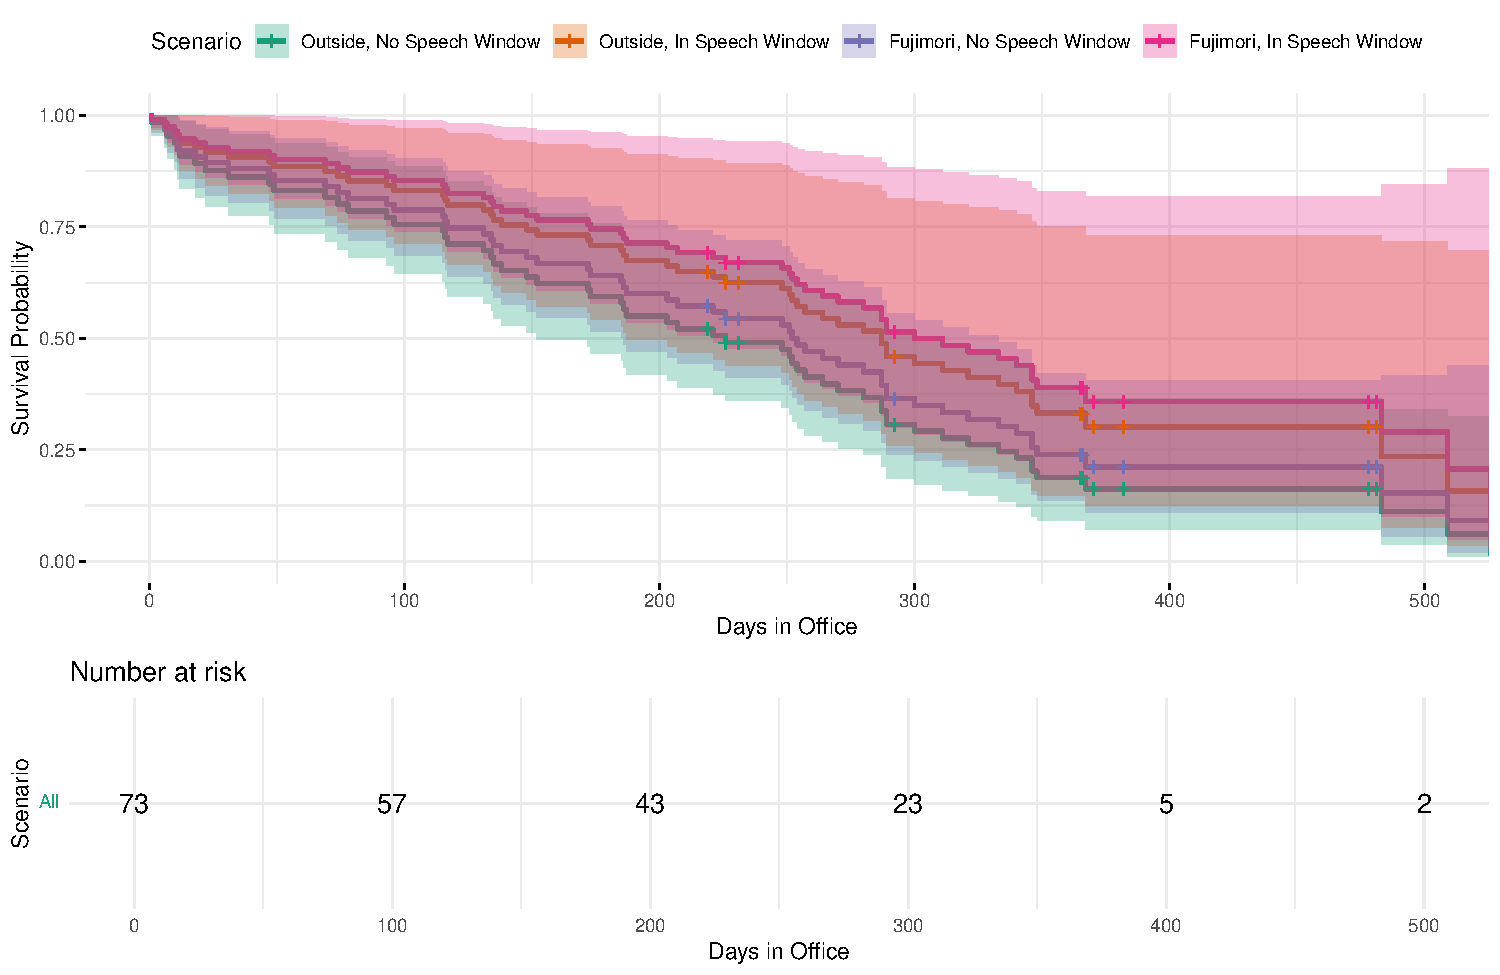
\includegraphics[width=0.85\textwidth]{combined_survival_plot.pdf}
% % \caption{Survival curves by scenario (Fujimori vs. Outside)}
% % \label{fig:survcurve}
% % \end{figure}
% 
% % \begin{sidewaysfigure}
%   \begin{figure}[ht]
%     \centering
%     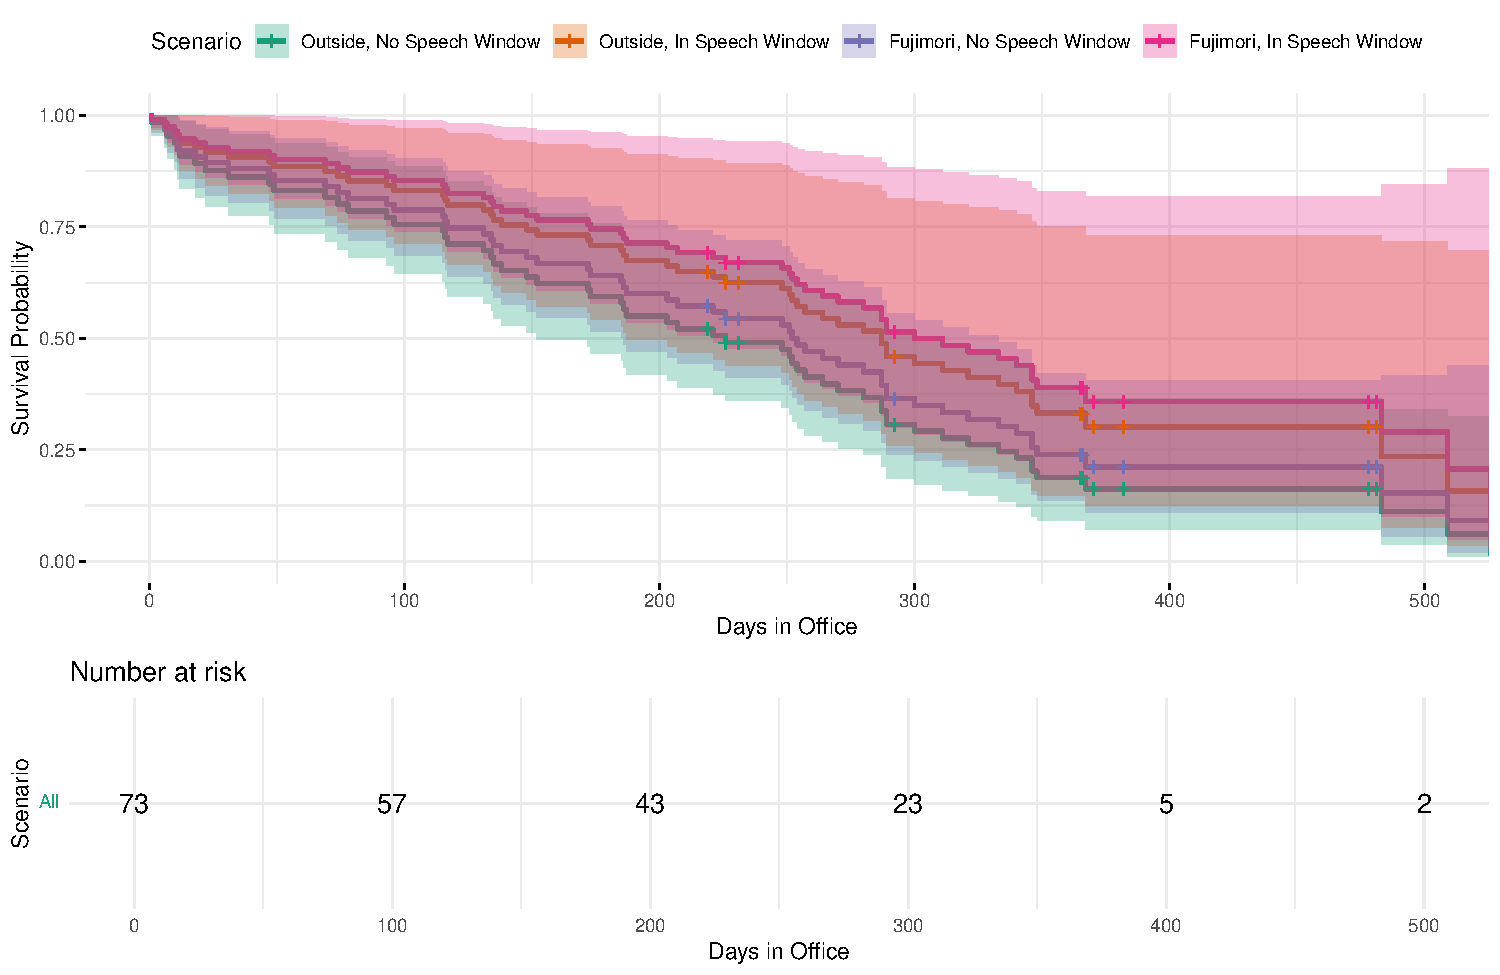
\includegraphics[width=\textwidth]{combined_survival_plot.pdf}
%     \caption{Estimated PCM survival curves under four scenarios: outside/in speech window and non‑Fujimori/Fujimori periods.}
%     \label{fig:survival_curves}
%   \end{figure}
% % \end{sidewaysfigure}
% 
% This plot shows four estimated survival curves—each with 95 \% confidence bands—derived from the simplified Cox model (no frailty) for combinations of the Fujimori regime dummy and the $\pm$ 45-day speech window:
% 
% \begin{itemize}
% \item Green (“Outside, No Speech Window”): PCM spells that start outside the speech window and outside the Fujimori period.
% 
% \item Orange (“Outside, In Speech Window”): Spells that start within ± 45 days of July 28 but outside Fujimori.
% 
% \item Blue (“Fujimori, No Speech Window”): Spells during Fujimori that start more than 45 days from the speech.
% 
% \item Pink (“Fujimori, In Speech Window”): Spells during Fujimori that start within the speech window.
% \end{itemize}
% 
% From this plot we can say that overall decline in survival. All curves drop from 1.0 toward 0 as days in office accumulate—by around 300 days only half of PCMs remain in office on average.
% 
% Regime effect (Fujimori vs. non-Fujimori): The two Fujimori curves (blue and pink) lie above their non-Fujimori counterparts, indicating longer average survival under Fujimori. For instance, at 200 days the survival probability is roughly 0.65 under Fujimori versus about 0.50 outside it.
% 
% Speech-window effect: Within each regime, the “in speech window” curve (orange and pink) tracks slightly above the “no speech window” curve (green and blue), suggesting a modest reduction in exit risk when a spell begins near the annual address date. This difference, however, is small relative to the CIs.
% 
% Precision declines over time: The shaded bands widen toward the right, reflecting increasing uncertainty as fewer spells survive into longer tenures. Beyond ~400 days, the confidence intervals become very wide, so point‐estimate differences at those durations are not very informative.
% 
% Number at risk: The table below shows how many intervals remain “at risk” at key time-points (0, 100, 200, … days). You start with 72 intervals (57 spells split at speech cut–points), dropping to just 2 intervals by ~500 days.
% 
% 
% Although the point estimates hint at better survival during Fujimori and slightly lower exit risk for spells initiated near the speech, these contrasts fall well within the wide confidence bands. This visual underscores why the minimal two-covariate model didn’t yield statistically significant regime or speech-window effects—and why adding the institutional (ENP), approval, and economic covariates is essential to sharpen the estimated drivers of PCM durability.
% 
% 
% 
% \section{Software and replication}
% 
% Models are estimated in R 4.3 using packages \emph{survival}, \emph{coxme}, and \emph{ggsurvfit}. All data and scripts are archived on Github
% 
% 
% \section{Conclusion}
% 
% \section{Apendixes}

% %%%%% adding bibliography
\bibliographystyle{apacite} %%style
\renewcommand{\refname}{Bibliography}
\bibliography{Premieres} %% filename

\end{document} %% nothing after here

